\documentclass[journal,12pt,twocolumn]{IEEEtran}

\usepackage{setspace}
\usepackage{gensymb}
\singlespacing
\usepackage[cmex10]{amsmath}

\usepackage{amsthm}

\usepackage{mathrsfs}
\usepackage{txfonts}
\usepackage{stfloats}
\usepackage{bm}
\usepackage{cite}
\usepackage{cases}
\usepackage{subfig}

\usepackage{longtable}
\usepackage{multirow}

\usepackage{enumitem}
\usepackage{mathtools}
\usepackage{steinmetz}
\usepackage{tikz}
\usepackage{circuitikz}
\usepackage{verbatim}
\usepackage{tfrupee}
\usepackage[breaklinks=true]{hyperref}
\usepackage{graphicx}
\usepackage{tkz-euclide}

\usetikzlibrary{calc,math}
\usepackage{listings}
    \usepackage{color}                                            %%
    \usepackage{array}                                            %%
    \usepackage{longtable}                                        %%
    \usepackage{calc}                                             %%
    \usepackage{multirow}                                         %%
    \usepackage{hhline}                                           %%
    \usepackage{ifthen}                                           %%
    \usepackage{lscape}     
\usepackage{multicol}
\usepackage{chngcntr}

\DeclareMathOperator*{\Res}{Res}

\renewcommand\thesection{\arabic{section}}
\renewcommand\thesubsection{\thesection.\arabic{subsection}}
\renewcommand\thesubsubsection{\thesubsection.\arabic{subsubsection}}

\renewcommand\thesectiondis{\arabic{section}}
\renewcommand\thesubsectiondis{\thesectiondis.\arabic{subsection}}
\renewcommand\thesubsubsectiondis{\thesubsectiondis.\arabic{subsubsection}}


\hyphenation{op-tical net-works semi-conduc-tor}
\def\inputGnumericTable{}                                 %%

\lstset{
%language=C,
frame=single, 
breaklines=true,
columns=fullflexible
}
\begin{document}


\newtheorem{theorem}{Theorem}[section]
\newtheorem{problem}{Problem}
\newtheorem{proposition}{Proposition}[section]
\newtheorem{lemma}{Lemma}[section]
\newtheorem{corollary}[theorem]{Corollary}
\newtheorem{example}{Example}[section]
\newtheorem{definition}[problem]{Definition}

\newcommand{\BEQA}{\begin{eqnarray}}
\newcommand{\EEQA}{\end{eqnarray}}
\newcommand{\define}{\stackrel{\triangle}{=}}
\bibliographystyle{IEEEtran}
\raggedbottom
\setlength{\parindent}{0pt}
\providecommand{\mbf}{\mathbf}
\providecommand{\pr}[1]{\ensuremath{\Pr\left(#1\right)}}
\providecommand{\qfunc}[1]{\ensuremath{Q\left(#1\right)}}
\providecommand{\sbrak}[1]{\ensuremath{{}\left[#1\right]}}
\providecommand{\lsbrak}[1]{\ensuremath{{}\left[#1\right.}}
\providecommand{\rsbrak}[1]{\ensuremath{{}\left.#1\right]}}
\providecommand{\brak}[1]{\ensuremath{\left(#1\right)}}
\providecommand{\lbrak}[1]{\ensuremath{\left(#1\right.}}
\providecommand{\rbrak}[1]{\ensuremath{\left.#1\right)}}
\providecommand{\cbrak}[1]{\ensuremath{\left\{#1\right\}}}
\providecommand{\lcbrak}[1]{\ensuremath{\left\{#1\right.}}
\providecommand{\rcbrak}[1]{\ensuremath{\left.#1\right\}}}
\theoremstyle{remark}
\newtheorem{rem}{Remark}
\newcommand{\sgn}{\mathop{\mathrm{sgn}}}
\providecommand{\abs}[1]{\left\vert#1\right\vert}
\providecommand{\res}[1]{\Res\displaylimits_{#1}} 
\providecommand{\norm}[1]{\left\lVert#1\right\rVert}
%\providecommand{\norm}[1]{\lVert#1\rVert}
\providecommand{\mtx}[1]{\mathbf{#1}}
\providecommand{\mean}[1]{E\left[ #1 \right]}
\providecommand{\fourier}{\overset{\mathcal{F}}{ \rightleftharpoons}}
%\providecommand{\hilbert}{\overset{\mathcal{H}}{ \rightleftharpoons}}
\providecommand{\system}{\overset{\mathcal{H}}{ \longleftrightarrow}}
	%\newcommand{\solution}[2]{\textbf{Solution:}{#1}}
\newcommand{\solution}{\noindent \textbf{Solution: }}
\newcommand{\cosec}{\,\text{cosec}\,}
\providecommand{\dec}[2]{\ensuremath{\overset{#1}{\underset{#2}{\gtrless}}}}
\newcommand{\myvec}[1]{\ensuremath{\begin{pmatrix}#1\end{pmatrix}}}
\newcommand{\mydet}[1]{\ensuremath{}}}
\numberwithin{equation}{subsection}

\makeatletter
\@addtoreset{figure}{problem}
\makeatother
\let\StandardTheFigure\thefigure
\let\vec\mathbf

\renewcommand{\thefigure}{\theproblem}

\def\putbox#1#2#3{\makebox[0in][l]{\makebox[#1][l]{}\raisebox{\baselineskip}[0in][0in]{\raisebox{#2}[0in][0in]{#3}}}}
     \def\rightbox#1{\makebox[0in][r]{#1}}
     \def\centbox#1{\makebox[0in]{#1}}
     \def\topbox#1{\raisebox{-\baselineskip}[0in][0in]{#1}}
     \def\midbox#1{\raisebox{-0.5\baselineskip}[0in][0in]{#1}}
\vspace{3cm}
\title{Gate Assignment 1}
\author{Tanmay Goyal - AI20BTECH11021}
\maketitle
\newpage
\bigskip
\renewcommand{\thefigure}{\theenumi}
\renewcommand{\thetable}{\theenumi}

Download all latex codes from 
\begin{lstlisting}
https://github.com/tanmaygoyal258/EE3900-Linear-Systems-and-Signal-processing/blob/main/GateAssignment1/main.tex
\end{lstlisting}
\section{Problem}
(EC 2017- Q.7) The input $x(t)$ and output $y(t)$ of a continous time signal are related as:
\begin{align}
    y(t) = \int_{t-T}^tx(u)\,du
\end{align}
The system is:
\begin{enumerate}
    \item Linear and Time-variant
    \item Linear and Time-invariant
    \item Non-Linear and Time-variant
    \item Non-Linear and Time-invariant
\end{enumerate}
\section{Solution}
A necessary and sufficient condition for the linearity of a system is to check if it follows the Principle of Superposition, i.e Law of Additivity and Law of Homogeneity.

\underline{Law of Additivity:}\\
Let the two input signals be $x_1(t)$ and $x_2(t)$, and their corresponding output signals be $y_1(t)$ and $y_2(t)$, then:
\begin{align}
    y_1(t) = \int_{t-T}^tx_1(u)\,du\\
    y_2(t) = \int_{t-T}^tx_2(u)\,du\\
    y_1(t) + y_2(t) = \int_{t-T}^t[x_1(u) + x_2(u)]\,du
    \label{1}
\end{align}
Now, consider the input signal of $x_1(t) + x_2(t)$, then the corresponding output signal is given by $y'(t)$:
\begin{align}
    y'(t) = \int_{t-T}^t[x_1(u) + x_2(u)]\,du
    \label{2}
\end{align}
Clearly, from \eqref{1} and \eqref{2}:
\begin{align}
    y'(t) = y_1(t) + y_2(t)
\end{align}
Thus, the Law of Additivity holds.\\

\underline{Law of Homogeneity: }\\
Consider an input signal $kx(t)$, where $k$ is any constant. Let the corresponding output be given by $y'(t)$, then:
\begin{align}
    y'(t) = \int_{t-T}^t kx(u)\,du\\
    = k\int_{t-T}^t x(u)\,du\\
     = ky(t)
     \label{3}
\end{align}
Clearly, from \eqref{3},
\begin{align}
    y'(t) = ky(t)
\end{align}
Thus, the Law of Homogeneity holds.\\

Since both the Laws hold, the system satisfies the Principle of Superposition, and is thus, a \textbf{linear system}.\\

To check for time-invariance, we would introduce a delay of $t_0$ in the output and input signals.\\
Delay in output signal:
\begin{align}
    y(t-t_0) = \int_{t-t_0-T}^{t-t_0} x(u)\,du
    \label{4}
\end{align}
Now, we consider an input signal with a delay of $t_0$, given by $x(t-t_0)$, and let the corresponding output signal be given by $y'(t)$, then:
\begin{align}
    y'(t) = \int_{t-T}^{t} x(u-t_0)\,du
\end{align}
Substituting $a = u-t_0$:
\begin{align}
    y'(t) = \int_{t-t_0-T}^{t-t_0} x(a)\,da
    \label{5}
\end{align}
Clearly, from \eqref{4} and \eqref{5}:
\begin{align}
    y'(t) = y(t-t_0)
\end{align}
Thus, the system is \textbf{time-invariant}.\\
The correct option is \textbf{2) Linear and Time-invariant}
\begin{figure}[!ht]
\centering
 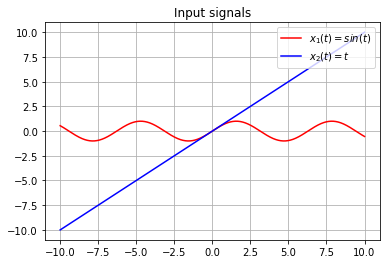
\includegraphics[width=\columnwidth]{graphs/input_signals.png}
 \caption{$x_1(t) = \sin{t}$ and $x_2(t) = t$}
 \end{figure}
\begin{figure}[!ht]
\centering
 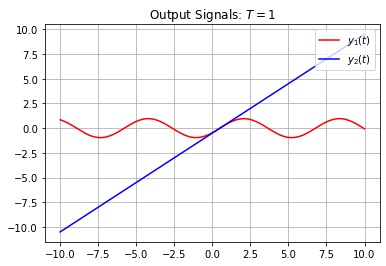
\includegraphics[width=\columnwidth]{graphs/output_signals.png}
 \caption{$y_1(t)$ and  $y_2(t)$}
 \end{figure}
 \begin{figure}[!ht]
\centering
 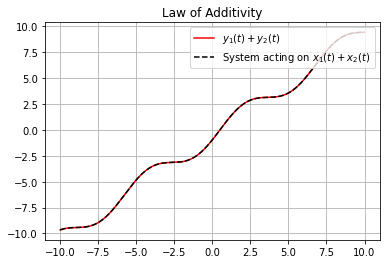
\includegraphics[width=\columnwidth]{graphs/law_of_additivity.png}
 \caption{Law of Additivity}
 \end{figure}
 \begin{figure}[!ht]
\centering
 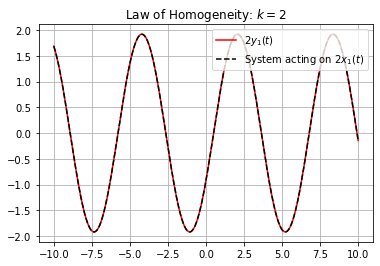
\includegraphics[width=\columnwidth]{graphs/law_of_homogeneity.png}
 \caption{Law of Homogeneity}
 \end{figure}
  \begin{figure}[!ht]
\centering
 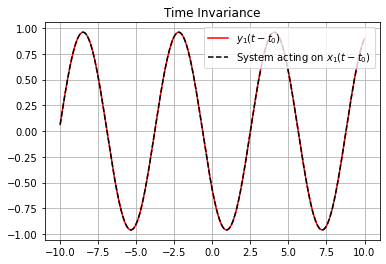
\includegraphics[width=\columnwidth]{graphs/time_invariance.png}
 \caption{Time invariance}
 \end{figure}
\end{document}